\section{Problema 3: La caja en el plano}

\subsection{Introducci\'on}

\indent En este caso, el problema que se nos presentó para resolver fue el siguiente:\\
\indent Se tienen $n$ puntos en el plano con coordenadas enteras y se tiene adem\'as una caja, representada por un rect\'angulo de dimensiones dada. La caja puede ubicarse en cualquier lugar del plano, pero no puede rotarse, es decir, la base de la caja debe quedar paralela al eje $x$ y la altura de la caja debe quedar paralela al eje $y$. Un punto sobre un borde de la caja se considera dentro de la misma. Se desea ubicar la caja de manera tal que la cantidad de puntos que queden dentro de la caja sea m\'axima. El algoritmo que resuelva este problema debe hacerlo con una complejidad de a lo sumo \textbf{O}($n^{3}$).\\
\indent Es oportuno realizar alguna aclaraciones. En primer lugar, que el problema siempre tiene soluci\'on \'optima, es decir que siempre habr\'a una ubicaci\'on de la caja que cubra mayor o igual cantidad de puntos que todas las dem\'as. En segundo lugar, que la soluci\'on \'optima no siempre es \'unica. \\
\indent A continuaci\'on se provee un ejemplo de una posible instancia del problema con una posible soluci\'on y que adem\'as sirve para mostrar las aclaraciones hechas anteriormente:\\


\begin{figure}[H]
	\centering
	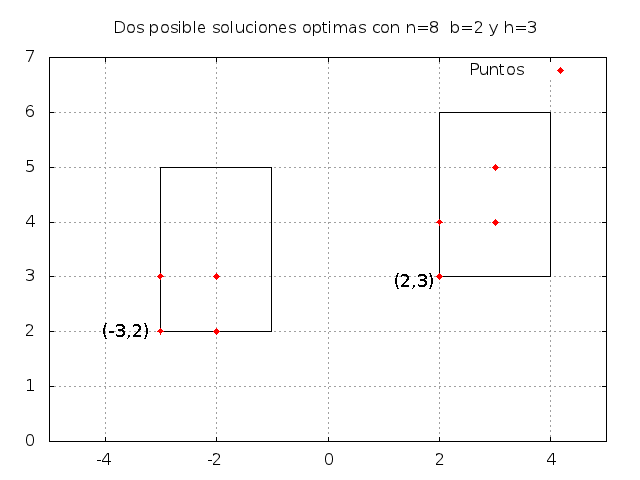
\includegraphics[scale=0.6]{ej3-grafico1.png}
	\caption{ Aqu\'i se observa como existe más de una soluci\'on \'optima para el problema, puesto que tanto $(-3,2)$ como $(2,3)$ cubren la m\'axima cantidad de puntos posibles, en este caso cuatro.}
\end{figure}


\indent Para resolver este problema hemos asumido que por lo menos se tiene alg\'un punto en el plano (es decir que $n>0$) y que adem\'as los puntos que se proveen por entrada no est\'an repetidos.\\

\subsection{Desarrollo}


\indent Dado el problema a resolver, la primera noci\'on que se extrajo al momento de analizarlo fue el hecho de que siempre existe una soluci\'on \'optima, aunque no siempre es \'unica.\\
\indent Una primera aproximaci\'on intuitiva para la resoluci\'on consisti\'o en ir posicionando la esquina inferior izquierda de la caja en todos los lugares posibles de un \'area acotada por cuatro puntos, cada uno el m\'as extremo hacia la izquierda, la derecha, arriba o abajo. Si bien parece l\'ogico encontrar la soluci\'on deseada de esta manera, el algoritmo ser\'ia muy complejo (y en particular la complejidad estar\'ia condicionada por la lejan\'ia entre los puntos extremos), por lo que resultaba necesario acotar de alguna manera las posibles posiciones donde se evaluar\'ia la esquina inferior izquierda de la caja.\\
\indent Una segunda aproximaci\'on consisti\'o en ir probando cada punto en los cuatro v\'ertices de la caja y evaluar cu\'antos de los dem\'as puntos entrar\'ian en ella. Sin embargo, esta idea no result\'o ser fruct\'ifera: solamente est\'abamos evaluando potenciales soluciones que cumpl\'ian con tener por lo menos un punto en el v\'ertice y no es cierto que siempre existe una soluci\'on \'optima que tenga por lo menos un punto en el v\'ertice.\\
\indent Luego de analizar m\'as detenidamente el contexto del problema, se comprendi\'o que a partir de un posicionamiento de la esquina inferior izquierda de la caja con la condici\'on de que por lo menos un punto quedara cubierto por ella, uno podr\'ia encontrar otro posicionamiento que cumpliera que por lo menos un punto cubierto por ella se encuentre en el borde inferior de la caja y otro en el borde izquierdo de la caja (puede darse el caso que sean el mismo punto, si es así el punto estar\'ia ubicado en el v\'ertice inferior izquierdo de la caja) y que la cantidad de puntos dentro de la caja de este posicionamiento es mayor o igual que la cantidad del primer posicionamiento.\\
 								
\begin{figure}[H]
	\centering
	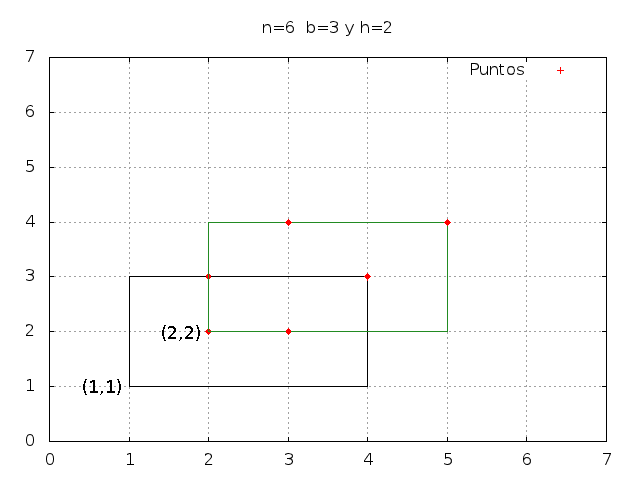
\includegraphics[scale=0.6]{ej3-grafico2.png}
	\caption{ Aqu\'i se observa como a partir de la posici\'on $(1,1)$ de una caja se puede hallar otra (la $(2,2)$ ) que tenga por lo menos un punto en el borde,los mismos puntos que la $(1,1)$ y que puede llegar a cubrir m\'as puntos. }
\end{figure}


\indent  De aqu\'i se extrae que siempre hay por lo menos una solución \'optima que cumpla con estos criterios, puesto que la soluci\'on \'optima debe cubrir por lo menos un punto. En particular, esa soluci\'on \'optima cumple con que el componente $x$ de su esquina inferior izquierda se corresponde con la coordenada $x$ de alguno de los puntos que se tienen en el plano y que el componente $y$ de su esquina inferior izquierda se corresponde con la coordenada $y$ de alguno de los puntos que se tienen en el plano (y que no necesariamente son el mismo punto).Una demostraci\'on de todo esto se puede encontrar en la secci\'on de Correctitud de este problema.\\
\indent De esta manera hemos reducido el conjunto de posibles soluciones a uno m\'as pequeño y que sabemos con seguridad que contiene una soluci\'on \'optima.\\ 
\indent Luego, las potenciales soluciones son las esquinas inferiores izquierdas que cumplen que su coordenada $x$ se corresponde con la componente $x$ de alguno de los puntos en el plano y que su coordenada $y$ se corresponde con la componente $y$ de alguno de los puntos en el plano.\\
\indent As\'i, hay a lo sumo $n^{2}$ candidatos a soluci\'on a analizar que se obtienen de combinar la coordenada $x$ de cada punto con las coordenadas $y$ de todos los puntos. En particular, nuestro algoritmo recorre estos candidatos a soluci\'on y devuelve el candidato que m\'as puntos cubra, siendo as\'i una soluci\'on \'optima.\\

\subsection{Algoritmo} 

\indent Queremos hacer un par de aclaraciones: $n$, $b$ y $h$ son de tipo $int$ y representan la cantidad de puntos, la base de la caja y la altura de la caja respectivamente. A su vez, puntosX contiene en la posici\'on $i$ la coordenada $x$ del i-\'esimo punto de la entrada. An\'alogamente, puntosY contiene en la posici\'on $i$ la coordenada $y$ del i-\'esimo punto de la entrada. Por lo tanto, la longitud de ambos vectores es $n$, la cantidad de puntos en el plano.\\
\indent Adem\'as queremos mencionar que, en caso de existir m\'as de una soluci\'on \'optima, la soluci\'on que devuelve el algoritmo est\'a fuertemente influenciada por el orden en el que se pasaron los puntos por la entrada. De esta manera se pueden pasar por entrada dos instancias iguales, con la \'unica diferencia del orden en el que se pasan los puntos, y el algoritmo devovlver dos soluciones distintas en cada instancia, siendo sin embargo las dos \'optimas.\\
\indent El algoritmo recorre los candidatos a soluci\'on que cumplen que su coordenada $x$ coincide con la de alg\'un punto del sistema y que su coordenada $y$ coincide con la de alg\'un punto del sistema (que puede no ser el mismo que el de la coordenada $x$).\\
\indent Esto se basa en el hecho de que en dicho conjunto de puntos seguro existe por lo menos una soluci\'on \'optima. Se provee la demostraci\'on de esta afirmaci\'on en la secci\'on Correctitud de este problema.\\


\begin{algorithm}[H]
\caption{} 
\begin{codebox}
\Procname{$\proc{resolver}(n, b, h, vector<int> puntosX, vector<int> puntosY)$}
\li int $cant \gets 0$
\li int $m \gets 0$
\li int $resx \gets puntosX[0]$
\li int $resy \gets puntosY[0]$
\li \For int $i$ desde 0 hasta n \Do
\li		\For int $j$ desde 0 hasta n \Do
\li 		$m \gets $ cuantosEntran(n, b, h, puntosX[i], puntosY[j], puntosX, puntosY)
\li 		\If $(cant<m)$ 
\li				\Then   $cant \gets m$
\li 					$resx \gets puntosX[i]$
\li 					$resy \gets puntosY[j]$
				\End
			\End
		\End
	\End
\li \Return $cant$ , $resx$, $resy$

\End
\end{codebox}
\end{algorithm}


\begin{algorithm}[H]
\caption{} 
\begin{codebox}
\Procname{$\proc{cuantosEntran}(n, b, h, x, y, vector<int> puntosX, vector<int> puntosY)$}
\li int $cant \gets 0$
\li \For int $i$ desde 0 hasta n \Do
\li 	\If ($(x \leq puntosX[i] \leq x+b)$  $AND$  $(y \leq puntosY[i] \leq x+h)$) \Do
\li 		$cant$ ++		
 		\End
 	\End	
\li \Return $cant $
\End
\end{codebox}
\end{algorithm}

\subsubsection{Correctitud}

\indent Sean $s$= ($s_{x}$,$s_{y}$) una coordenada entera que representa la esquina inferior izquierda de la caja, $P$ el conjunto de los puntos en el plano, $n$ la cantidad de puntos en el plano, $b$ la base de la caja y $h$ la altura de la caja. Y sea $P_{s}$=\{$p_{1}...p_{k}$\} el conjunto de los puntos que quedan cubiertos por la caja cuya esquina inferior izquierda est\'a en $s$.\\

\indent Definimos una soluci\'on \'optima para este problema como aquel $s$ que cumple que $\#(P_{s}) \geq \#(P_{r}) $ para todo $r$ coordenada entera.\\

\indent En primer lugar, veamos que $\exists$ un $t$ soluci\'on \'optima tal que $t_{x} = e_{x}$ $\wedge$ $t_{y}=f_{y}$ para algunos $e,f \in P$ (no es necesario que $e=f$).\\

\indent Para ello, veamos que siempre existe una soluci\'on \'optima con por lo menos un punto en el borde de la caja.\\

%\indent Sea $s$ una coordenada. Supongamos $P_{s}=\{$p_{1}...p_{k}$\}\neq \emptyset$, es decir que la caja representada por $s$ cubre por lo menos un punto.\\
%\indent Para todo $p \in P_{s}$ vale que \\
%\begin{center}
%$s_{x} \leq p_{x} \leq s_{x} + b$  $\wedge$ \\
%$s_{y} \leq p_{y} \leq s_{y} + h$\\
\end{center}\\

puesto que est\'an cubiertos por la caja.\\

\indent Ahora bien, sean $a = \min_{i:1...k}((p_{i})_{x})$ y $c = \min_{i:1...k}((p_{i})_{y})$.\\
\indent Definamos ahora $s$' tal que $s'_{x} = a$ $\wegde$ $s'_{y}=c $.\\
\indent Entonces, para todo $i$ desde 1 hasta $k$:\\
\begin{center}
$s'_{x} = a = \min_{i:1...k}((p_{i})_{x}) \leq (p_{i})_{x}$  $\wedge$ \\
$s'_{y} = c = \min_{i:1...k}((p_{i})_{y}) \leq (p_{i})_{y}$  \\
\end{center}\\

\indent Es decir,\\ 

\begin{center}
$s'_{x} \leq p_{x}$  $\wedge$ \\
$s'_{y} \leq p_{y}$  \\
\end{center}\\
 
para todo $p \in P_{s}$ .\\

\indent Adem\'as, por como definimos $s'$:\\
\begin{center}
$s_{x} \leq s'_{x} $  $\wedge$ \\
$s_{y} \leq s'_{y}$\\
\end{center}\\

\indent Por lo tanto, para todo $p \in P_{s}$:\\
\begin{center}
$s_{x} \leq s'_{x} \leq p_{x} \leq s_{x} + b  \leq s'_{x} + b$  $\wedge$ \\
$s_{y} \leq s'_{y} \leq p_{y} \leq s_{y} + h  \leq s'_{y} + h$\\
\end{center}\\

\indent Es decir que:\\
\begin{center}
$s'_{x} \leq p_{x} \leq s'_{x} + b$  $\wedge$ \\
$s'_{y} \leq p_{y} \leq s'_{y} + h$\\
\end{center}\\

y eso quiero decir que para todo punto $p \in P_{s} $ vale que $ p \in P_{s'}$. \\
\indent Luego, $P_{s} \subseteq P_{s'}.$\\
\indent Es decir que $\#P_{s} \leq \#P_{s'}$. \\
\indent Notar que no vale la vuelta, puesto que al reubicar la caja se pueden estar cubriendo puntos que antes no estaban cubiertos.\\
									
\indent En particular, si $s$ es una soluci\'on \'optima, vale que $\#(P_{s}) \geq \#(P_{r}) $ para todo $r$ coordenada entera (recordamos que en la plano hay por lo menos un punto y que necesariamente la soluci\'on \'optima tiene que cubrir por lo menos un punto).\\
\indent Luego, $\#P_{s} \geq \#P_{s'}$. Pero como $\#P_{s} \leq \#P_{s'}$, entonces:\\

\begin{center}
$\#P_{s} = \#P_{s'}$
\end{center}\\

y entonces $s'$ tambi\'en es soluci\'on \'optima. Como siempre se puede encontrar una soluci\'on \'optima $s$, entonces tambi\'en siempre se puede encontrar una soluci\'on \'optima $s'$. Es decir que hemos encontrado una soluci\'on \'optima que cumple que tiene por lo menos un punto en el borde.\\

\indent Definamos ahora el conjunto de coordenadas\\
\begin{center}
$Z = \{z | z_{x}= e_{x} $ para alg\'un $e \in P$  $\wedge$ $z_{y}= f_{y}$ para alg\'un $f \in P\}$
\end{center}\\

\indent Es decir que $Z$ es el conjunto de coordenadas que cumplen que su componente $x$ se corresponde con el de alg\'un punto en el plano y que su componente $y$ se corresponde con la alg\'un punto en el plano (no necesariamente el mismo punto).\\

\indent Es fácil observar que de la manera en que lo definimos, $s' \in Z $.\\ 
\indent Esto es porque $s'_{x} =  \min_{p \in P_{s'}}(p_{x})$  $\wedge$  $s'_{y} =  \min_{p \in P_{s'}}(p_{y})$. \\
\indent  Adem\'as como siempre puedo encontrar un $s'$ con estas condiciones que sea soluci\'on \'optima, eso quiere decir que seguro existe una soluci\'on \'optima en $Z$.\\
\indent Por lo tanto, $\exists$ una coordenada $t$ soluci\'on \'optima tal que $t_{x} = e_{x}$ $\wedge$ $t_{y}=f_{y}$ para algunos $e,f \in P$ (no es necesario que $e=f$), que es lo que quer\'iamos demostrar.\\


\indent Ahora veamos como nuestro algoritmo encuentra una soluci\'on correcta.\\
\indent Es f\'acil ver que en efecto el conjunto $Z$ se puede formar combinando las componentes $x$ de cada punto en el plano con las componentes $y$ de los todos puntos en el plano. Como ya hemos demostrado, en ese conjunto seguro hay alguna soluci\'on \'optima $s$ que en particular cumple que para todo $z \in Z$  $\#P_{s} \geq \#P_{z}$. \\
\indent El algoritmo recorre entonces todos los elementos $z$ del conjunto $Z$. Mediante la funci\'on  $cuantosEntran$ se cuenta la cantidad de puntos que entran en la caja que tiene como esquina inferior izquierda a $z$, es decir que devuelve $\#P_{z}$  y lo conserva como soluci\'on parcial si y sólo si es la que mayor puntos cubre hasta ese momento.Es decir que en cada iteraci\'on la soluci\'on parcial (llam\'emosla $v$) cumple que $\#P_{v}$ es mayor que la todos los puntos $z$ que se evaluaron hasta ese momento.\\
\indent Luego, cuando se iteraron todos los elementos de $Z$ la soluci\'on $s$ que tenemos cumple que $\#P_{s} \geq \#P_{z}$ para todo $z \in Z$.\\
\indent Pero como sabemos que en ese conjunto existe una soluci\'on \'optima, entonces $s$ tambi\'en lo es. En particular, lo que puede ocurrir es que devuelva esa soluci\'on \'optima que demostramos que existe en el conjunto $Z$ (es decir la que tiene puntos en los bordes de la caja) o que devuelva otra que no cumpla con esa condici\'on, pero que al cumplir que $\#P_{s} \geq \#P_{z} $ tambi\'en es soluci\'on \'optima.\\

\indent \indent \indent \indent \indent \indent \indent \indent \indent \indent \indent \indent \indent \indent  \indent \indent $\square$




\subsubsection{Análisis de Complejidad}

\indent Analicemos en primer lugar la complejidad de $cuantosEntran$. Asignarle un valor a la variable $int$ $cant$ cuesta tiempo constante, es decir \textbf{O}(1). A su vez, evaluar la condición del If también cuesta tiempo constante.Esto es porque realizar la comparaci\'on de $int$'s es constante y, de acuerdo a la documentaci\'on de C++, obtener un elemento de un vector mediante el operador [] tambi\'en lo es. Por lo tanto, evaluar la condición del If es \textbf{O}(1). Luego, se entre o no al cuerpo del If, en cada iteraci\'on del ciclo se ejecuta algo de costo constante. Como el ciclo se itera $n$ veces (siendo $n$ la cantidad de puntos que hay en el plano), el algoritmo $cuantosEntran$ tiene un costo de\\
\begin{center}
\textbf{O}(1 + n*1)
\end{center}\\

con lo cual tiene una complejidad temporal \textbf{O}(n), es decir lineal en la cantidad de puntos.\\


\indent Analicemos ahora $resolver$. Las primeras cuatro asignaciones se realizan en tiempo constante (incluso las que obtienen un valor del vector con el operador [ ]), es decir en \textbf{O}(1).\\
\indent Veamos que ocurre en el cuerpo del segundo For. Se ejecuta $cuantosEntran$, que ya sabemos que lo hace en tiempo lineal, y lo que devuelve se lo asigna a una variable (en tiempo constante). Luego se hace una comparaci\'on en \textbf{O}(1).\\
\indent Ahora bien, si no entra al cuerpo del If no se hace nada más y se pasa a la pr\'oxima iteraci\'on. En este caso el costo de la iteración fue de \textbf{O}(n+2), con lo cual tiene una complejidad temporal de \textbf{O}(n).\\
\indent En cambio, si entra al cuerpo del If, se realizan tres asignaciones, todas en tiempo constante. Luego lo que está adentro del cuerpo del If tiene un costo de \textbf{O}(1). Es decir que en este caso también una iteraci\'on cuesta \textbf{O}(n).\\
\indent De aqu\'i se extrae que lo que ocurre en cada iteraci\'on de este For tiene un costo lineal. Como este For se ejecuta $n$ veces, su complejidad temporal será \textbf{O}($n^2$).\\
\indent Entonces, el primer For ejecuta en cada iteración algo con un costo cuadrático. Como se itera $n$ veces se obtiene que el costo de este For es \textbf{O}($n^3$). Es decir que el algoritmo cuesta \\
\begin{center}
\textbf{O}(1+1+1+ n^3)
\end{center}\\

con lo cual tiene un complejidad temporal de \textbf{O}($n^3$), es decir c\'ubica en la cantidad de puntos, cumpliendo entonces con la cota que se nos exigía en el enunciado del problema.\\


\subsection{Pruebas y Resultados}

\indente Primero queremos realizar una aclaraci\'on. Por la manera en que implementamos el algoritmo, no es esperable un caso patol\'ogico. Esto es porque el algoritmo siempre itera en las $n^2$ combinaciones posibles que se obtienen de las componentes $x$ e $y$ de todos los puntos. Quiz\'a es oportuno mencionar que esto se podr\'ia optimizar generando un vector de combinaciones y quitando los elementos repetidos. En este caso, si para todo par de puntos de la entrada vale que tienen coordenadas $x$ e $y$ distintas, ese vector de combinaciones ser\'ia de tamaño $n^$.\\
\indent Se realizaron casos de prueba de manera aleatoria. El programa permite la creaci\'on se estos casos de prueba si as\'i lo quisiese el usuario.  En particular, se crearon tres archivos de entrada generados de manera aleatoria que se pueden encontrar en la misma carpeta que el c\'odigo fuente. Cada uno de estos archivos contempla casos que contienen desde un punto hasta doscientos. A partir de estos tres archivos, y utilizando la funci\'on $get_clocktime()$, se lograron obtener los tiempos de ejecuci\'on para cada eso. Con estos datos se confeccionaron los siguientes gr\'aficos que relacionan el tiempo de ejecuci\'on del algoritmo con la cantidad de puntos en el plano:\\

\begin{figure}[H]
	\centering
	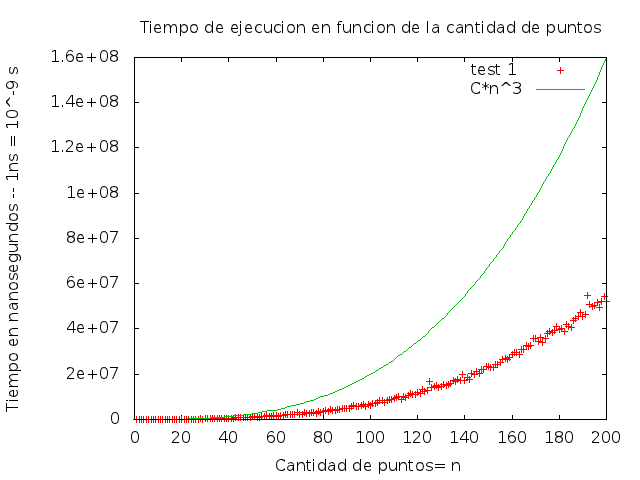
\includegraphics[scale=0.6]{ej3-test1.png}
	\caption{Gr\'afico de tiempo de ejecuci\'on en funci\'on de la cantidad de puntos para el archivo de entrada $testingAzar1.txt$ comparada con la cota te\'orica O($n^3$) }
\end{figure}

\begin{figure}[H]
	\centering
	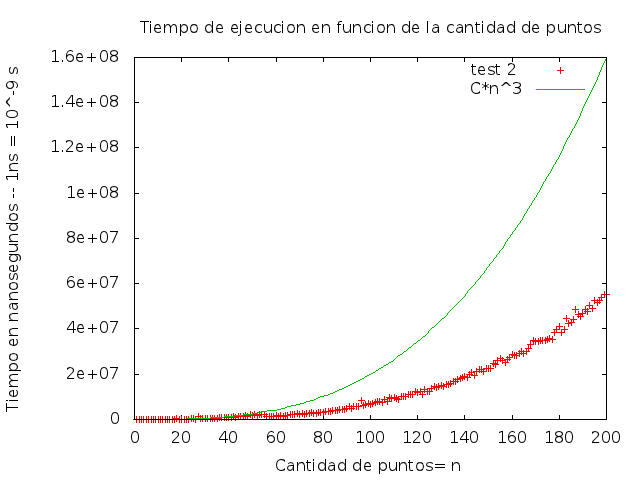
\includegraphics[scale=0.5]{ej3-test2.png}
	\caption{ Gr\'afico de tiempo de ejecuci\'on en funci\'on de la cantidad de puntos para el archivo de entrada $testingAzar2.txt$ comparada con la cota te\'orica O($n^3$)}
\end{figure}

\begin{figure}[H]
	\centering
	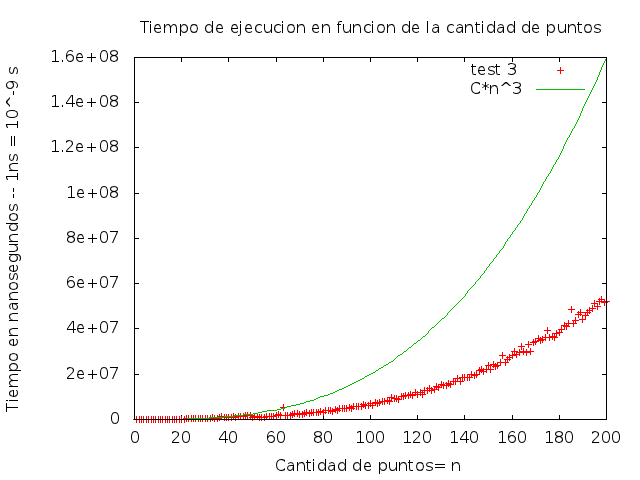
\includegraphics[scale=0.5]{ej3-test3.png}
	\caption{ Gr\'afico de tiempo de ejecuci\'on en funci\'on de la cantidad de puntos para el archivo de entrada $testingAzar3.txt$ comparada con la cota te\'orica O($n^3$)}
\end{figure}

\indent De estos gr\'aficos se puede extraer que los tres casos aleatorios parecen cumplir con la cota te\'orica c\'ubica que hab\'iamos conjeturado. Es decir que a partir de alg\'un valor de $n$ todos las mediciones de tiempo se ajustan de la curva $C*n^3$ que representa a la cota te\'orica.\\


\begin{figure}[H]
	\centering
	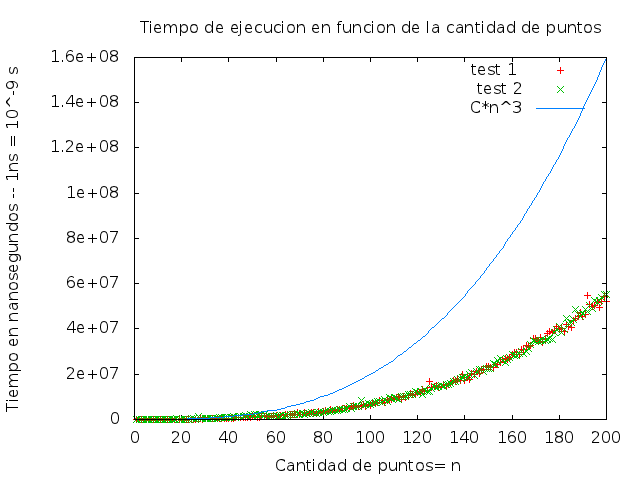
\includegraphics[scale=0.5]{ej3-compTestAzarEj3.png}
	\caption{ Gr\'afico de comparativo del tiempo de ejecuci\'on en funci\'on de la cantidad de puntos para los archivos de entrada $testingAzar1.txt$ y $testingAzar2.txt$ comparada con la cota te\'orica O($n^3$)}
\end{figure}

\indent Este gr\'afico expone que fijado un $n$ los tiempos de ejecuci\'on para dos instancias del problema parecen comportarse en cuanto a tiempo de ejecuci\'on de maneras similares. No se provey\'o un gr\'afico que comparase los tres archivos de entradas aleatorias en favor de la visualizaci\'on del gr'afico.\\

\subsection{Conclusiones}

\indent Se concluye que el algoritmo parece responder de la forma esperada en cuanto a performance temporal se refiere, cumpliendo con la cota te\'orica \textbf{O}($n^3$). Además, a trav\'es de los casos de testing estudiados, se deduce que fijada una cantidad de puntos $n$ dos intancias con dicho valor de $n$ se ejecutan en tiempos similares.\\ 


